%!TEX root = ../main.tex
\section{Ορισμός}

Με τον όρο Computer Vision αναφερόμαστε στο διεπιστημονικό πεδίο που ασχολείται με τον τρόπο με τον οποίο μπορούν να κατασκευαστούν υπολογιστές για την επίτευξη υψηλής κατανόησης από ψηφιακές εικόνες και βίντεο. Από την άποψη της μηχανικής, είναι οι τρόποι για την επίτευξη της αυτοματοποίησης εργασιών που μπορούν να πραγματοποιηθούν από την ανθρώπινη όραση. \cite{wiki:Computer_vision}

Τα καθήκοντα της υπολογιστικής όρασης περιλαμβάνουν μεθόδους απόκτησης, επεξεργασίας, ανάλυσης και κατανόησης ψηφιακών εικόνων και εξαγωγής δεδομένων από τον πραγματικό κόσμο με σκοπό την παραγωγή αριθμητικών ή συμβολικών πληροφοριών. όπως για παράδειγμα στην μορφή λήψης αποφάσεων.

Η κατανόηση σε αυτό το πλαίσιο ταυτίζεται με τη μετατροπή των οπτικών εικόνων σε περιγραφές του κόσμου που μπορούν να αλληλεπιδρούν με άλλες διαδικασίες σκέψης και να διεγείρουν τις κατάλληλες ενέργειες.

Αυτή η κατανόηση των εικόνων μπορεί να θεωρηθεί ως η απεμπλοκή συμβολικών πληροφοριών από δεδομένα εικόνας χρησιμοποιώντας μοντέλα κατασκευασμένα με τη βοήθεια της γεωμετρίας, της φυσικής, των στατιστικών και της θεωρίας της μάθησης. Από τη σκοπιά της επιστήμης, η μηχανική όραση ασχολείται με τη θεωρία πίσω από τα τεχνητά συστήματα που εξάγουν πληροφορίες από εικόνες.

Τα δεδομένα αυτά μπορούν να λάβουν πολλαπλές μορφές όπως ακολουθίες βίντεο, προβολές από πολλές κάμερες ή πολυδιάστατα δεδομένα από ιατρικό σαρωτή. Από την σκοπιά της τεχνολογίας όμως, επιδιώκει να εφαρμόσει τις θεωρίες και τα μοντέλα για την κατασκευή συστημάτων ηλεκτρονικής όρασης.

Οι υποτομείς της μηχανικής όρασης περιλαμβάνουν την αναδημιουργία σκηνών, την ανίχνευση συμβάντων, την παρακολούθηση βίντεο, την αναγνώριση αντικειμένων, την εκτίμηση θέσης 3D, τη μάθηση, την εκτίμηση κίνησης και την αποκατάσταση της εικόνας.
\begin{figure}[H]
  	\centering
	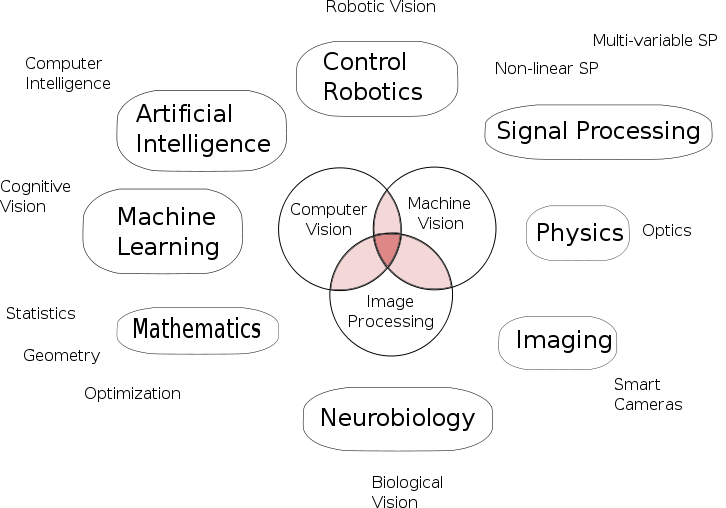
\includegraphics[width=0.65\textwidth]{images/CV}\\
	\caption{Υπολογιστική όραση \& σχετικοί τομείς \cite{wiki:Glossary_of_machine_vision}}
\end{figure}
\section{Ιστορική αναδρομή}

Στα τέλη της δεκαετίας του 1960, η μηχανική όραση ξεκίνησε σε πανεπιστήμια πρωτοπόρα στην τεχνητή νοημοσύνη. Σκοπός ήταν να μιμείται το ανθρώπινο οπτικό σύστημα, ως ένα ένα ενδιάμεσο βήμα για να προσδώσει έξυπνη συμπεριφορά σε ρομπότ. Αυτό που διαφοροποίησε τη υπολογιστική όραση από τον επικρατέστερο τομέα της ψηφιακής επεξεργασίας εικόνων ήταν η επιθυμία να εξαχθεί τρισδιάστατη δομή από εικόνες με στόχο την επίτευξη πλήρους κατανόησης της σκηνής. Μελέτες στη δεκαετία του '70 αποτέλεσαν τα θεμέλια για πολλούς από τους αλγορίθμους υπολογιστικής όρασης που χρησιμοποιούνται ακόμη και τώρα, συμπεριλαμβανομένης της εξαγωγής ακμών από εικόνες, σήμανσης γραμμών, μη πολυεδρικής και πολυεδρικής μοντελοποίησης, αναπαράστασης αντικειμένων ως διασυνδέσεων μικρότερων δομών, οπτικής ροής και εκτίμηση κίνησης.

Την επόμενη δεκαετία πραγματοποιήθηκαν μελέτες βασισμένες σε πιο αυστηρές μαθηματικές αναλύσεις και ποσοτικές πτυχές της μηχανικής όρασης. Οι ερευνητές συνειδητοποίησαν επίσης ότι πολλές μαθηματικές έννοιες θα μπορούσαν να αντιμετωπιστούν εντός του ίδιου πλαισίου βελτιστοποίησης όπως για παράδειγμα η κανονικοποίηση και τα τυχαία πεδία Markov. Μέχρι τη δεκαετία του 1990, μερικά από τα προηγούμενα ερευνητικά θέματα έγιναν πιο ενεργά από τα υπόλοιπα. Η έρευνα σε 3D-ανακατασκευές οδήγησε σε καλύτερη κατανόηση της βαθμονόμησης της κάμερας. Με την εμφάνιση των μεθόδων βελτιστοποίησης για τη βαθμονόμηση της κάμερας, διαπιστώθηκε ότι πολλές από τις ιδέες είχαν ήδη εξερευνηθεί στη θεωρία προσαρμογής δέσμης από το πεδίο της φωτογραμμετρίας. Αυτό οδήγησε σε μεθόδους για αραιές 3-D ανακατασκευές σκηνών από πολλές εικόνες.
Αυτή η δεκαετία σηματοδότησε επίσης την πρώτη φορά που οι τεχνικές στατιστικής μάθησης χρησιμοποιήθηκαν στην πράξη για την αναγνώριση προσώπων στις εικόνες.

Προς τα τέλη της δεκαετίας του 1990, σημαντική αλλαγή επήλθε με την αυξημένη αλληλεπίδραση μεταξύ των πεδίων των γραφικών και της μηχανικής όρασης. Αυτό περιελάμβανε απεικόνιση με βάση την εικόνα, μορφοποίηση εικόνας, παρεμβολή προβολής, ραφή πανοραμικών εικόνων και απόδοση φωτεινού πεδίου. Πρόσφατα, έχει παρατηρηθεί αναζωπύρωση σε μεθόδους βασισμένες σε χαρακτηριστικά, που χρησιμοποιούνται σε συνδυασμό με τεχνικές machine learning και περίπλοκα frameworks βελτιστοποίησης.

\section{Εφαρμογές}

Οι εφαρμογές της υπολογιστικής όρασης κυμαίνονται από την ανάπτυξη συστημάτων βιομηχανικής μηχανικής όρασης έως τη διερεύνηση τεχνητής νοημοσύνης και ανάπτυξη ρομπότ και ηλεκτρονικών υπολογιστών ικανών να κατανοήσουν τον κόσμο τριγύρω τους. Τα πεδία της υπολογιστικής όρασης και μηχανικής όρασης έχουν σημαντική αλληλεπικάλυψη. Η υπολογιστική όραση καλύπτει τη βασική τεχνολογία της αυτοματοποιημένης ανάλυσης εικόνας που χρησιμοποιείται σε πολλά πεδία.

Η μηχανική όραση αναφέρεται συνήθως σε μια διαδικασία συνδυασμού της αυτοματοποιημένης ανάλυσης εικόνας με άλλες μεθόδους και τεχνολογίες για την παροχή αυτοματοποιημένης επιθεώρησης και καθοδήγησης ρομπότ σε βιομηχανικές εφαρμογές. Σε πολλές εφαρμογές υπολογιστικής όρασης, οι υπολογιστές έχουν προ-προγραμματιστεί για την επίλυση μια συγκεκριμένης εργασίας αλλά οι μέθοδοι που βασίζονται στη μάθηση γίνονται ολοένα συχνότερες. Παραδείγματα εφαρμογής της υπολογιστικής όρασης περιλαμβάνουν συστήματα για:
\begin{itemize}
	\item Αυτοματοποιημένη επιθεώρηση, πχ σε βιομηχανικές εφαρμογές, γραμμές παραγωγής
	\item Παροχή βοήθειας στους ανθρώπους σε εργασίες αναγνώρισης
	\item Διαδικασίες ελέγχου
	\item Ανίχνευση συμβάντων
	\item Αλληλεπίδραση, πχ ως είσοδος σε μια συσκευή αλληλεπίδρασης ανθρώπου-μηχανής
	\item Μοντελοποίηση αντικειμένων
	\item Πλοήγηση, πχ σε αυτόνομα οχήματα
	\item Οργάνωση πληροφοριών \\
\end{itemize}

Ένα από τα σημαντικότερα πεδία εφαρμογής της υπολογιστικής όρασης είναι αυτό της ιατρικής υπολογιστικής όρασης. Αυτός ο τομέας χαρακτηρίζεται από την εξαγωγή πληροφοριών από δεδομένα εικόνας με σκοπό την πραγματοποίηση ιατρικής διάγνωσης ενός ασθενούς. Γενικότερα, τα δεδομένα έχουν τη μορφή μικροσκοπικών εικόνων, εικόνων ακτίνων X, αγγειογραφικών εικόνων, εικόνων υπερήχου και εικόνων τομογραφίας. Από δεδομένα τέτοιου τύπου μπορεί να εξαχθεί ένα μεγάλο πλήθος δεδομένων όπως για παράδειγμα, η ανίχνευση όγκων, αρτιοσκλήρυνσης κα. Είναι δυνατή επίσης η μέτρηση των διαστάσεων των οργάνων, της ροής αίματος κλπ.

Οι στρατιωτικές εφαρμογές είναι ίσως μία από τις μεγαλύτερες περιοχές της υπολογιστικής όρασης. Τα προφανή παραδείγματα είναι η ανίχνευση εχθρικών στρατιωτών ή οχημάτων και καθοδήγηση πυραύλων. Τα πιο προηγμένα συστήματα για την καθοδήγηση πυραύλων στέλνουν τον πύραυλο σε μια περιοχή αντί για έναν συγκεκριμένο στόχο και η επιλογή στόχου γίνεται όταν ο πύραυλος φτάσει στην περιοχή με βάση τα τοπικά δεδομένα εικόνας. Οι σύγχρονες στρατιωτικές έννοιες, όπως η `συνειδητοποίηση των πεδίων μάχης', υποδηλώνουν ότι διάφοροι αισθητήρες, συμπεριλαμβανομένων των αισθητήρων εικόνας, παρέχουν μια πλούσια συλλογή πληροφοριών σχετικά με μια σκηνή μάχης που μπορεί να χρησιμοποιηθεί για τη στήριξη στρατηγικών αποφάσεων. Στην περίπτωση αυτή, η αυτόματη επεξεργασία των δεδομένων χρησιμοποιείται για να μειώσει την πολυπλοκότητα και να συγχωνεύσει πληροφορίες από πολλούς αισθητήρες για να αυξήσει την αξιοπιστία.
\section{Μέθοδοι συστήματος υπολογιστικής όρασης}

Η οργάνωση ενός συστήματος ηλεκτρονικής όρασης εξαρτάται σε μεγάλο βαθμό από την εφαρμογή. Ορισμένα συστήματα είναι αυτόνομες εφαρμογές που επιλύουν ένα συγκεκριμένο πρόβλημα μέτρησης ή ανίχνευσης, ενώ άλλα αποτελούν ένα υποσύστημα μεγαλύτερου σχεδιασμού το οποίο περιλαμβάνει για παράδειγμα υποσυστήματα για τον έλεγχο μηχανικών ενεργοποιητών, προγραμματισμό, βάσεις δεδομένων, μηχανικές διεπαφές κλπ. Η συγκεκριμένη εφαρμογή ενός συστήματος υπολογιστικής όρασης εξαρτάται επίσης από το εάν η λειτουργικότητά του είναι προκαθορισμένη ή αν κάποιο μέρος του μπορεί να μάθει ή να τροποποιηθεί κατά τη λειτουργία. Πολλές λειτουργίες είναι μοναδικές για την εφαρμογή. Υπάρχουν, ωστόσο, τυπικές λειτουργίες που εντοπίζονται σε πολλά συστήματα ηλεκτρονικής όρασης.
\begin{itemize}
	\item \textbf{Συλλογή εικόνας} - Μια ψηφιακή εικόνα παράγεται από έναν ή περισσότερους αισθητήρες εικόνας. Ανάλογα με τον τύπο του αισθητήρα η εικόνα μπορεί να είναι είτε μία 2D εικόνα, είτε 3D. Μπορεί επίσης να είναι μια ακολουθία εικόνων.
	\item \textbf{Προεπεξεργασία} - Προτού να μπορεί να εφαρμοστεί μια μέθοδος ηλεκτρονικής όρασης σε δεδομένα εικόνας ώστε να εξαχθεί κάποια συγκεκριμένη πληροφορία, είναι συνήθως απαραίτητη η επεξεργασία των δεδομένων προκειμένου να διασφαλιστεί ότι ικανοποιεί ορισμένες υποθέσεις που υποδηλώνει η μέθοδος. Για παράδειγμα:
	\begin{itemize}
		\item Επαναδειγματοληψία
		\item Μείωση θορύβου
		\item Βελτίωση αντίθεσης
	\end{itemize}
	\item \textbf{Εξαγωγή χαρακτηριστικών} - Χαρακτηριστικά της εικόνας σε διάφορα επίπεδα πολυπλοκότητας εξάγονται από τα δεδομένα της. Τυπικά παραδείγματα τέτοιων χαρακτηριστικών είναι:
	\begin{itemize}
		\item Γραμμές, ακμές και κορυφογραμμές
		\item Σημεία τοπικού ενδιαφέροντος όπως γωνίες, κηλίδες ή σημεία
	\end{itemize}
	\item \textbf{Ανίχνευση / τμηματοποίηση} - Σε κάποιο σημείο της επεξεργασίας λαμβάνεται απόφαση σχετικά με το ποια σημεία εικόνας ή περιοχές της εικόνας είναι χρήσιμα για περαιτέρω επεξεργασία
	\begin{itemize}
		\item Επιλογή συγκεκριμένου συνόλου σημείων ενδιαφέροντος
		\item Τμηματοποίηση μιας ή πολλαπλών περιοχών εικόνας που περιέχουν ένα συγκεκριμένο αντικείμενο ενδιαφέροντος
	\end{itemize}
	\item \textbf{Επεξεργασία υψηλού επιπέδου} - Σε αυτό το βήμα η είσοδος είναι συνήθως ένα μικρό σύνολο δεδομένων, για παράδειγμα ένα σύνολο σημείων ή μια περιοχή εικόνας που υποτίθεται ότι περιέχει ένα συγκεκριμένο αντικείμενο. Η υπόλοιπη επεξεργασία αφορά, για παράδειγμα:
	\begin{itemize}
		\item Επαλήθευση ότι τα δεδομένα ικανοποιούν παραδοχές που βασίζονται σε μοντέλα και εφαρμογές
		\item Εκτίμηση συγκεκριμένων παραμέτρων της εφαρμογής
		\item Αναγνώριση εικόνων
		\item Καταχώρηση εικόνας
	\end{itemize}
	\item \textbf{Λήψη αποφάσεων} - Πραγματοποιείται η τελική απόφαση που απαιτεί η εφαρμογή όπως για παράδειγμα:
	\begin{itemize}
		\item \textbf{Pass / fail} στις εφαρμογές αυτόματης επιθεώρησης
		\item \textbf{Match / no match} σε εφαρμογές αναγνώρισης
		\item \textbf{Flag} για περαιτέρω επιθεώρηση από άνθρωπο
	\end{itemize}
\end{itemize}
\section{Υπολογιστική όραση \& FPGAs}

Η πολυπλοκότητα των αλγορίθμων υπολογιστικής όρασης σε συνδυασμό με τη συνεχώς αυξανόμενη ζήτηση για εφαρμογές με τεράστια μεγέθη δεδομένων όπως για παράδειγμα εικόνες ή βίντεο υψηλής ανάλυσης, έχει οδηγήσει στην ανάγκη για μεγάλη υπολογιστική ισχύ. Οι επεξεργαστές γενικού σκοπού καθώς και σε αρκετές περιπτώσεις οι GPUs δε μπορούν να ικανοποιήσουν τις απαιτήσεις ισχύος. Συνεπώς, συστήματα όπως ASICs αποκτούν σημαντικό πλεονέκτημα στον τομέα της παρεχόμενης απόδοσης σε realtime εφαρμογές. Η προσέγγιση με ASICs όμως παρουσιάζει αρκετές δυσκολίες: το κόστος είναι υψηλό, ο σχεδιασμός τους είναι χρονοβόρος και μη επαναδιαμορφώσιμος μετά την κατασκευή τους.

Το γεγονός όμως ότι τα FPGA μπορούν να επαναδιαμορφώνονται τα κάνει κατάλληλα για αυτού του είδους εφαρμογές, ξεπερνώντας τους περιορισμούς που επιβάλλονται με τη χρήση των ASICs. Οι πρόσφατες βελτιώσεις στην τεχνολογία των FPGA σημαίνουν ότι μπορούν να επιτύχουν πολύ υψηλή απόδοση, κοντά στα επίπεδα των ASICs. Η ταυτόχρονη εκτέλεση των εντολών των επαναδιαμορφώσιμων συστήματων τα καθιστά πλέον κατάλληλα για την υλοποίηση αλγορίθμων υπολογιστικής όρασης. Για παράδειγμα, μία από τις συνηθέστερες διεργασίες σε αλγορίθμους ψηφιακής επεξεργασίας εικόνας ή σήματος είναι η συνέλιξη. Πολλά συστήματα μηχανικής όρασης χρησιμοποιούν δισδιάστατη συνέλιξη με πυρήνες μετασχηματισμών ($3\times 3$, $5\times 5$) για την εφαρμογή φίλτρων σε εικόνες με σκοπό την αναγνώριση ακμών κα. Σε έναν επεξεργαστή γενικού σκοπού, αυτού του είδους οι διεργασίες είναι χρονοβόρες απαιτώντας εκατομμύρια πολλαπλασιασμούς και προσθέσεις αλλά στα FPGA μπορεί να εκτελεστούν ταυτόχρονα.


